\section{Experiments}

\subsection{Input data}
To test the correctness of the algorithms we used the MONK's datasets. To use these datasets correctly we did the following steps:
\begin{itemize}
	\item We preprocessed MONK's datasets with \textit{1-of-k} encoding to convert categorical data to numerical data and we obtained 17 binary input features vectors. This preprocessing is divided between two classes, \textit{Preprocessing} and \textit{LoadDataset}. The former reads, shuffle and split the dataset whereas the latter performs the \textit{1-to-k} encoding. 
	\item To view all the network in vector formulation terms and exploit the \textit{Armadillo} numerical library, we performed batch computation by loading and transposing the entire dataset in a single matrix. The labels were split and saved in another matrix to compute the \textit{MSE} (sez \ref{Loss:Mse}) after the forward phase. To reduce the cost of moving matrices we took advantage of the \textit{move} operator available since C++11. 
	\item Our library can deal with classification and regression tasks exploiting the composition of the \textit{Layer} class.  So we implemented \textit{sigmoid} and \textit{linear} activation functions for the output layer and \textit{hyperbolic tangent} activation function for the hidden layers.
\end{itemize}



To obtain a deterministic behaviour of the algorithms, we used the entire MONKS datasets as the input of the network. We obtained three matrices that had dimensions: 124x18 (Monk 1), 169x17 (Monk 2), and 122x17 (Monk 3). To compare the behaviour of the algorithms, we collected three parameters for every epoch: the error of the network (in our case MSE), the norm of the gradient and the computational time spent on completing the epoch. These three parameters were used to make the convergence speed, residual and computational time plots shown below. For a better visualization of the plots the y-axis is plotted on a logarithmic scale (except for section 3.3 "Rate of convergence") and an enlargement version of each plots is shown aside. Before showing the plots a table with all the configurations used and the values obtained is shown.

\subsection{Configuration tested}
The notation $f^*$ specifies the optimal value reached by a specific configuration of the problem (that can includes the regularization term if it is used). 


\begin{center}
	\small\addtolength{\tabcolsep}{-3pt}
		\centering
		\begin{longtable}{|c|c|c|c|c|c|c|c|c|}
			\hline
			\textbf{Task}& \textbf{Optimizer}&\textbf{Iteration} & \textbf{L rate} & \multicolumn{1}{l|}{\textbf{Lambda}} & \textbf{Mom} & \textbf{$f^{*}$}& \textbf{$\Vert \nabla f_{k}\Vert$ }& \textbf{Time(ms)}\\ \hline 
			Monk1 & MDA & 900 & 0.9 & 0  & 0 & 8.67e-3 & 3.450e-1 & 267 \\
			Monk1 & MDA & 900 & 0.9 & 0  & 0.3 & 2.458e-3 & 1.390e-1 & 231 \\
			Monk1 & MDA & 900 & 0.9 & 0  & 0.6 & 7.535e-4 & 5.0557e-1 & 233 \\
			Monk1 & MDA & 900 & 0.9 & 0  & 0.9 & 1.159e-4 & 8.59058e-3 & 405 \\
			Monk1 & NMDA & 900 & 0.9 & 0  & 0 & 8.678e-2 & 3.450e-1 & 279 \\
			Monk1 & NMDA & 900 & 0.9 & 0  & 0.3 & 2.426e-3 & 1.381-e1 & 265 \\
			Monk1 & NMDA & 900 & 0.9 & 0  & 0.6 & 7.472e-4 & 5.093e-1 & 222 \\
			Monk1 & NMDA & 900 & 0.9 & 0  & 0.9 & 1.124e-4 & 8.992e-3 & 208 \\
			Monk1 & L-BFGS & 50 & - & 0  & 0 & 11e-15 & 784e-13 & 3267 \\
			Monk1 & L-BFGS & 50 & - & 3e-4  & 0 & 6.396e-2 & 1.134e-1 & 3623 \\
			Monk1 & L-BFGS & 50 & - & 5e-4  & 0 & 8.553e-2 & 9.089e-1 & 3733 \\
			Monk1 & L-BFGS & 50 & - & 7e-4  & 0 & 1.201e-1 & 1.245e-1 & 5943 \\
			Monk1 & PBM & 400 & - & 0  & 0 & 6.962e-6 & 7.510e-4 & 29642 \\
			Monk1 & PBM & 400 & - & 3e-4  & 0 & 8.114e-1 & 7.510e-4 & 26849 \\
			Monk1 & PBM & 400 & - & 5e-4  & 0 & 1.352e-1 & 7.510e-4 & 27618 \\
			Monk1 & PBM & 400 & - & 7e-4  & 0 & 1.893e-1 & 7.510e-4 & 28247 \\
			Monk2 & MDA & 900 & 0.9 & 0  & 0 & 7.946e-2 & 5.151e-1 & 148\\
			Monk2 & MDA & 900 & 0.9 & 0  & 0.3 & 2.374e-2 & 3.236e-1 & 1128 \\
			Monk2 & MDA & 900 & 0.9 & 0  & 0.6 & 1.332e-2 & 8.083e-2 & 119 \\
			Monk2 & MDA & 900 & 0.9 & 0  & 0.9 & 6.673e-4 & 3.102e-2 & 342\\
			Monk2 & NMDA & 900 & 0.9 & 0  & 0 & 7.946e-2 & 5.151e-1 & 116\\
			Monk2 & NMDA & 900 & 0.9 & 0  & 0.3 & 2.486e-2 & 3.802e-1 & 179\\
			Monk2 & NMDA & 900 & 0.9 & 0  & 0.6 & 1.380e-2 & 9.093e-2 & 116\\
			Monk2 & NMDA & 900 & 0.9 & 0  & 0.9 & 1.403e-4 & 1.382e-2 & 939\\
			Monk2 & L-BFGS & 50 & - & 0  & 0 & 7.6e-14 & 3.788e-12 & 5610\\
			Monk2 & L-BFGS & 50 & - & 3e-4  & 0  & 5.919e-2 & 9.413e-2 & 5324\\
			Monk2 & L-BFGS & 50 & - & 5e-4  & 0  & 1.156e-1& 4.682e-1 & 6142\\
			Monk2 & L-BFGS & 50 & - & 7e-4  & 0  & 8.965e-2 &  4.468e-1 & 10047\\
			Monk2 & PBM & 400 & - & 0  & 0 & 3.453e-6 & 3.365e-4 & 37746\\
			Monk2 & PBM & 400 & - & 3e-4  & 0 & 1.211e-1 & 3.365e-4 & 37129\\
			Monk2 & PBM & 400 & - & 5e-4  & 0 & 2.018e-1 & 3.365e-4 & 39902\\
			Monk2 & PBM & 400 & - & 7e-4  & 0 & 2.825e-1 & 3.365e-4 & 37130\\
			Monk3 & MDA & 900 & 0.9 & 0  & 0 & 1.968e-2 & 3.236e-2 & 280\\
			Monk3 & MDA & 900 & 0.9 & 0  & 0.3 & 1.864e-2 & 2.297e-2 & 131\\
			Monk3 & MDA & 900 & 0.9 & 0  & 0.6 & 1.754e-2 & 1.301e-2 & 105\\
			Monk3 & MDA & 900 & 0.9 & 0  & 0.9 & 1.254e-2 & 7.248e-3 & 142\\
			Monk3 & NMDA & 900 & 0.9 & 0  & 0 & 1.968e-2 & 3.236e-2 & 106\\
			Monk3 & NMDA & 900 & 0.9 & 0  & 0.3 & 1.863e-2 & 2.277e-2 & 129\\
			Monk3 & NMDA & 900 & 0.9 & 0  & 0.6 & 1.754e-2 & 1.267e-2 & 300\\
			Monk3 & NMDA & 900 & 0.9 & 0  & 0.9 & 1.254e-2 & 7.139e-3 & 189\\
			Monk3 & L-BFGS & 50 & - & 0  & 0 & 8.196e-3 & 1.068e-12 & 8319\\
			Monk3 & L-BFGS & 50 & - & 3e-4  & 0  & 5.781e-2 & 3.603e-1 & 7947\\
			Monk3 & L-BFGS & 50 & - & 5e-4  & 0  & 8.555e-2 & 1.895e-1 & 12729\\
			Monk3 & L-BFGS & 50 & - & 7e-4  & 0  & 7.940e-2 & 1.525e-1 & 10153\\
			Monk3 & PBM & 400 & - & 0  & 0 & 1.231e-2 & 8.410e-4 & 35543\\
			Monk3 & PBM & 400 & - & 3e-4  & 0 & 7.988e-2 & 8.410e-4 & 35239\\
			Monk3 & PBM & 400 & - & 5e-4  & 0 & 1.249e-1 & 8.410e-4 & 35924\\
			Monk3 & PBM & 400 & - & 7e-4  & 0 & 1.699e-1 & 8.410e-4 & 35003\\
			\hline
			\caption{Network configurations with $f^*$.}
			\label{tab:nets_res}
		\end{longtable}

\end{center}

The table \ref{tab:nets_comp} contains the configurations of the networks used to obtain the plots in section \ref{sec:gradient_norm_convergence_speed}, section \ref{sec:rate_of_convergence}, section \ref{sec:computational_time} and \ref{sec:residual_error}. 

\begin{center}
	\small\addtolength{\tabcolsep}{-3pt}
	\centering
	\begin{longtable}{|c|c|c|c|c|c|c|c|c|}
		\hline
		\textbf{Task}& \textbf{Optimizer} & \textbf{L rate} & \multicolumn{1}{l|}{\textbf{Lambda}} & \textbf{Mom}  \\ \hline 
		Monk1 & MDA & 0.9 & - & 0.9    \\
		Monk1 & L-BFGS & - & 0 & -    \\
		Monk1 & PBM & - & 0 & -    \\
		Monk2 & MDA & 0.9 & - & 0.9    \\
		Monk2 & L-BFGS & - & 0 & -    \\
		Monk2 & PBM & - & 0 & -    \\
		Monk3 & MDA & 0.9 & - & 0.9    \\
		Monk3 & L-BFGS & - & 0 & -    \\
		Monk3 & PBM & - & 0 & -    \\
		\hline
		\caption{Network configurations used for the comparison plot.}
		\label{tab:nets_comp}
	\end{longtable}
\end{center}


\subsubsection{Methods minima analysis} 

As mentioned in \S\ref{LF:convexity}, the objective function is not convex. For this reason, we try to understand if the methods used were approaching the same optimal value or different ones.
First of all, we analysed the $f^{*}$ value of each configuration to understand at which optimal value the algorithms converge. 

\begin{longtable}{|c|c|c|c|c|c|}
	\hline
	\centering
	\textbf{Optimizer}&\textbf{Iteration} & \textbf{L rate} & \multicolumn{1}{l|}{\textbf{Lambda}} & \textbf{Mom} & \textbf{$f^{*}$} \\ \hline 
	L-BFGS & 50 & - & 0  & 0 & 11e-15  \\
	PBM & 400 & - & 0  & 0 & 6.962e-6 \\
	NMDA & 900 & 0.9 & 0  & 0.9 & 1.124e-4  \\
	MDA & 900 & 0.9 & 0  & 0.9 & 1.159e-4 \\
	NMDA & 900 & 0.9 & 0  & 0.6 & 7.472e-4  \\
	MDA & 900 & 0.9 & 0  & 0.6 & 7.535e-4 \\
	NMDA & 900 & 0.9 & 0  & 0.3 & 2.426e-3 \\
	MDA & 900 & 0.9 & 0  & 0.3 & 2.458e-3 \\
	MDA & 900 & 0.9 & 0  & 0 & 8.67e-3 \\
	L-BFGS & 50 & - & 3e-4  & 0 & 6.396e-2 \\
	L-BFGS & 50 & - & 5e-4  & 0 & 8.553e-2 \\
	NMDA & 900 & 0.9 & 0  & 0 & 8.678e-2 \\
	L-BFGS & 50 & - & 7e-4  & 0 & 1.201e-1 \\
	PBM & 400 & - & 5e-4  & 0 & 1.352e-1  \\
	PBM & 400 & - & 7e-4  & 0 & 1.893e-1  \\
	PBM & 400 & - & 3e-4  & 0 & 8.114e-1  \\
	\hline
	\caption{Monk 1 optimizer configuration displayed in increasing order of $f^*$.}
	\label{tab:nets_res_plots_Monk1}
\end{longtable}

As can be seen from table \ref{tab:nets_res_plots_Monk1} the different configuration of the optimizers MDA and NMDA with 900 iterations converge to the same optimal values. This can be stated because their optimal values differ between 3e-6 and 6e-6. Also for the L-BFGS optimizer with 5e-4 as regularization parameter using 50 iterations and the NMDA with 0.0 as momentum parameter using 900 iterations the optimal value differs of 1e-3.

\begin{longtable}{|c|c|c|c|c|c|}
	\hline
	\centering
	\textbf{Optimizer}&\textbf{Iteration} & \textbf{L rate} & \multicolumn{1}{l|}{\textbf{Lambda}} & \textbf{Mom} & \textbf{$f^{*}$} \\ \hline
	L-BFGS & 50 & - & 0  & 0 & 7.6e-14 \\
	PBM & 400 & - & 0  & 0 & 3.453e-6 \\ 
	NMDA & 900 & 0.9 & 0  & 0.9 & 1.403e-4 \\
	MDA & 900 & 0.9 & 0  & 0.9 & 6.673e-4 \\ 
	MDA & 900 & 0.9 & 0  & 0.6 & 1.332e-2 \\ 
	NMDA & 900 & 0.9 & 0  & 0.6 & 1.380e-2 \\ 
	MDA & 900 & 0.9 & 0  & 0.3 & 2.374e-2  \\ 
	NMDA & 900 & 0.9 & 0  & 0.3 & 2.486e-2 \\ 
	L-BFGS & 50 & - & 3e-4  & 0  & 5.919e-2 \\ 
	MDA & 900 & 0.9 & 0  & 0 & 7.946e-2 \\ 
	NMDA & 900 & 0.9 & 0  & 0 & 7.946e-2 \\ 
	L-BFGS & 50 & - & 7e-4  & 0  & 8.965e-2 \\ 
	L-BFGS & 50 & - & 5e-4  & 0  & 1.156e-1\\ 
	PBM & 400 & - & 3e-4  & 0 & 1.211e-1 \\  
	PBM & 400 & - & 5e-4  & 0 & 2.018e-1 \\ 
	PBM & 400 & - & 7e-4  & 0 & 2.825e-1 \\ 
	\hline
		\caption{Monk 2 optimizer configuration displayed in increasing order of $f^*$.}
	\label{tab:nets_res_plots_Monk2}
\end{longtable}

\begin{longtable}{|c|c|c|c|c|c|}
	\hline
	\centering
	\textbf{Optimizer}&\textbf{Iteration} & \textbf{L rate} & \multicolumn{1}{l|}{\textbf{Lambda}} & \textbf{Mom} & \textbf{$f^{*}$} \\ \hline 
	L-BFGS & 50 & - & 0  & 0 & 8.196e-3 		\\
	PBM & 400 & - & 0  & 0 & 1.231e-2 			\\
	PBM & 400 & - & 5e-4  & 0 & 1.249e-1 		\\
	MDA & 900 & 0.9 & 0  & 0.9 & 1.254e-2 	\\
	NMDA & 900 & 0.9 & 0  & 0.9 & 1.254e-2 	\\
	PBM & 400 & - & 7e-4  & 0 & 1.699e-1 		\\
	MDA & 900 & 0.9 & 0  & 0.6 & 1.754e-2 	\\
	NMDA & 900 & 0.9 & 0  & 0.6 & 1.754e-2 	\\
	NMDA & 900 & 0.9 & 0  & 0.3 & 1.863e-2 	\\
	MDA & 900 & 0.9 & 0  & 0.3 & 1.864e-2 	\\
	MDA & 900 & 0.9 & 0  & 0 & 1.968e-2 		\\
	NMDA & 900 & 0.9 & 0  & 0 & 1.968e-2 	\\
	L-BFGS & 50 & - & 3e-4  & 0  & 5.781e-2 	\\
	L-BFGS & 50 & - & 7e-4  & 0  & 7.940e-2 	\\
	PBM & 400 & - & 3e-4  & 0 & 7.988e-2 		\\
	L-BFGS & 50 & - & 5e-4  & 0  & 8.555e-2 	\\
	\hline
		\caption{Monk 3 optimizer configuration displayed in increasing order of $f^*$.}
	\label{tab:nets_res_plots_Monk3}
\end{longtable}

 Moreover, the $f^{*}$ values for the Monk1, Monk2 and Monk3 datasets are really close to each other for MDA and NMDA optimization algorithms. For Monk1, the $f^{*}$ values in L-BFGS algorithm with 3e-4 and 5e-4 as regularization parameter are close to each other, also $f^{*}$ values of L-BFGS with 7e-4 as regularization parameter is close to PBM $f^{*}$ values with 5e-4 and 7e-4 as regularization parameter. Similar behaviour can be found in Monk2. For Monk 3, there is different behaviour in which L-BFGS $f^{*}$ values with regularization are all close to each other and PBM with 3e-4 as regularization parameter is close to L-BFGS values. We observed that the L-BFGS converges to better values of the function in each problem. After further analysis, we observed that the weights initialization influences the  optimal values reached by all the networks after the optimization process.



\subsubsection{Rate of convergence}
\label{sec:rate_of_convergence}
To compute the rate of convergence for each algorithm, we consider $\alpha$ as the minimum residuals obtained by each of the optimization algorithm (that are the $f^{*}$ obtained for each configuration) and $f(x_{k})$ as the residual obtained at the iteration $k$ plus the regularization term if it is used. If exists a real positive constant $\gamma$ such that
\begin{equation}
\label{eq:rofFirst}
lim_{k\to \infty}\frac{|f(x_{k+1}) - \alpha |}{|f(x_{k}) - \alpha|^p} = \gamma > 0,
\end{equation}
we can state that the sequence of values $f(x_{k})$ produced by the algorithm has an order of convergence $p$. In our case, we can derive an alternative faster and rapid procedure to compute it. Considering the equation \ref{eq:rofFirst} we can obtain the following formula: 
\begin{equation}
p = lim_{k\to \infty}\frac{log |f(x_{k+1}) - \alpha | - log \gamma}{log|f(x_{k}) - \alpha|} \approx lim_{k\to \infty}\frac{log |f(x_{k+1}) - \alpha |}{log|f(x_{k}) - \alpha|}.
\end{equation}
If $p=1$ the convergence is linear and if $p=2$ the convergence is quadratic. We can observe in figure \ref{CR-Monk2} that L-BFGS reached a superlinear rate of convergence. 
As we expect from the analysis we made, L-BFGS reached a superlinear convergence rate in some epoch. Also for the Momentum Descent Approach, we see that the convergence rate obtained is linear as we expected. Instead, for the Proximal Bundle method we had some convergences rate peaks that we didn't expect. In our opinion, this can be caused by the particular loss shape of Monks dataset.
It's interesting to view that all of these methods even with a noisy dataset as Monk 3 converge with the same convergence rate as mentioned in the theory.

\begin{figure}[H]
	\centering
	\begin{minipage}[t]{0.5\linewidth}
		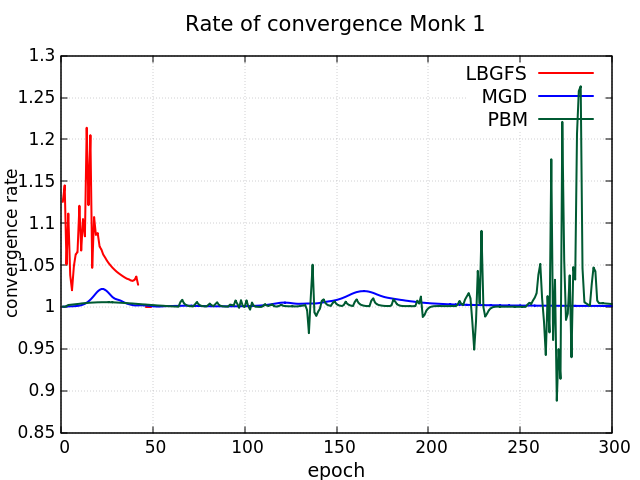
\includegraphics[width=\linewidth]{data/Comparison/Monk1/Monk1_CR_standard.png}
		\subcaption{Standard}
	\end{minipage}%
	\begin{minipage}[t]{0.5\linewidth}
		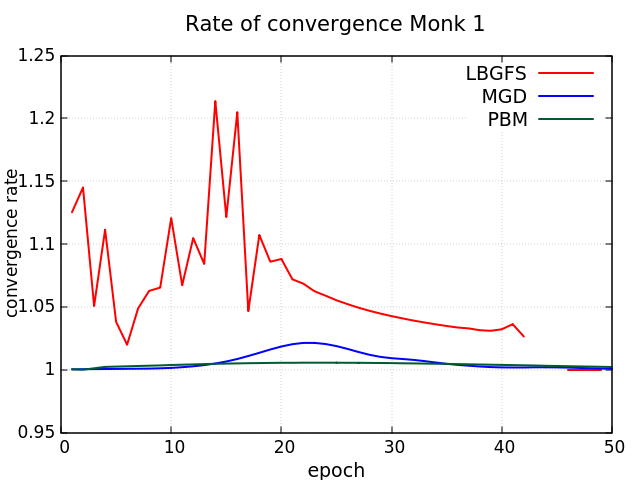
\includegraphics[width=\linewidth]{data/Comparison/Monk1/Monk1_CR_zoom.png}
		\subcaption{Zoom}
	\end{minipage}
	\caption{Converge rate comparison Monk 1 of configurations defined in table \ref{tab:nets_comp}}
	\label{CR-Monk1}
\end{figure}
\begin{figure}[H]
	\centering
	\begin{minipage}[t]{0.5\linewidth}
		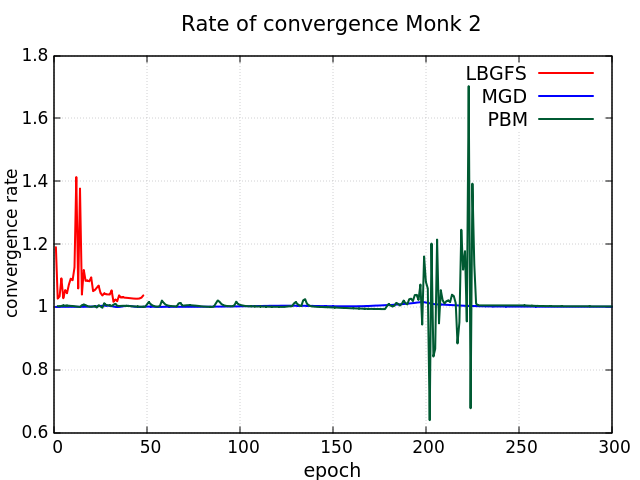
\includegraphics[width=\linewidth]{data/Comparison/Monk2/Monk2_CR_standard.png}
		\subcaption{Standard}
	\end{minipage}%
	\begin{minipage}[t]{0.5\linewidth}
		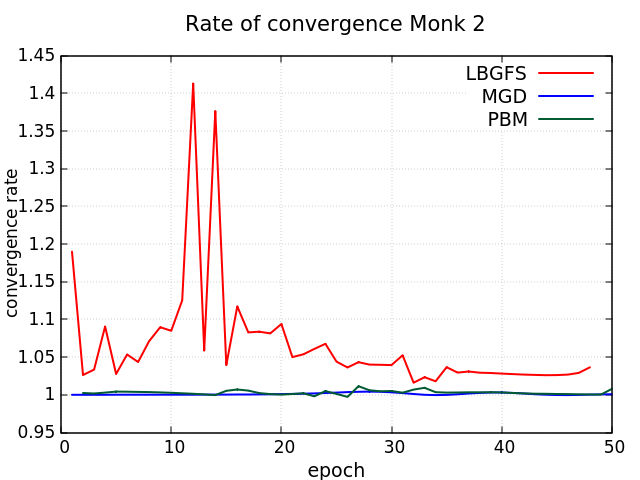
\includegraphics[width=\linewidth]{data/Comparison/Monk2/Monk2_CR_zoom.png}
		\subcaption{Zoom}
	\end{minipage}
	\caption{Converge rate comparison Monk 2 of configurations defined in table \ref{tab:nets_comp}}
	\label{CR-Monk2}
\end{figure}
\begin{figure}[H]
	\centering
	\begin{minipage}[t]{0.5\linewidth}
		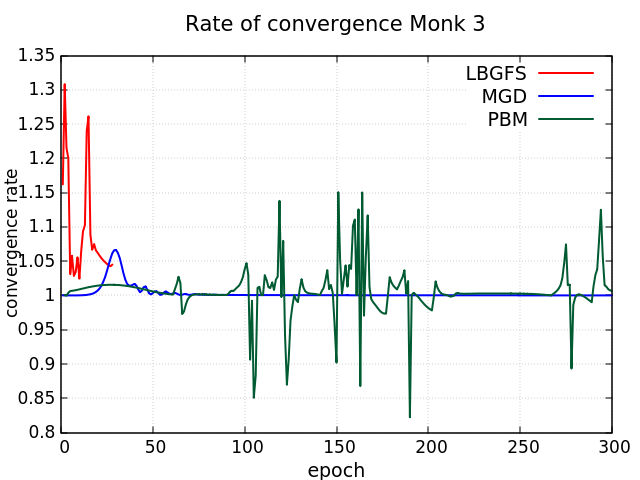
\includegraphics[width=\linewidth]{data/Comparison/Monk3/Monk3_CR_standard.png}
		\subcaption{Standard}
	\end{minipage}%
	\begin{minipage}[t]{0.5\linewidth}
		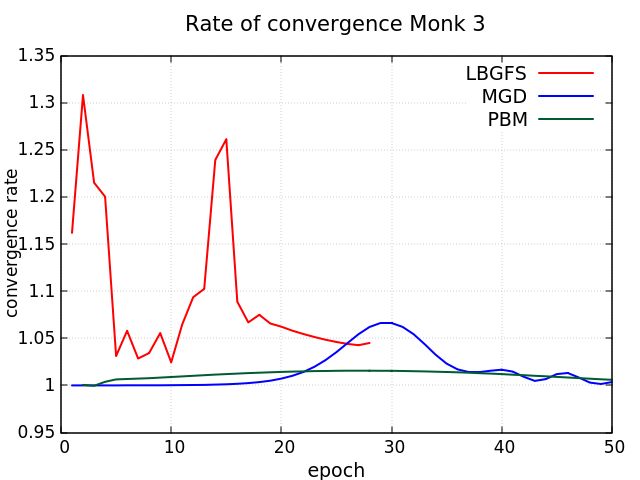
\includegraphics[width=\linewidth]{data/Comparison/Monk3/Monk3_CR_zoom.png}
		\subcaption{Zoom}
	\end{minipage}
	\caption{Converge rate comparison Monk 3 of configurations defined in table \ref{tab:nets_comp}}
	\label{CR-Monk3}
\end{figure}

\subsubsection{Computational time}
\label{sec:computational_time}
To compare the computational time behaviour of the implemented algorithm, we decided to display their curves in the plots \ref{CT-Monk1},\ref{CT-Monk2}, and \ref{CT-Monk3}. We can observe that, as expected from the theory, the most expensive method is the Proximal Bundle Method because of the time spent on the resolution of a quadratic programming problem by an external solver. As we can see in table \ref{tab:nets_res} the computational time of the Momentum Descent Approach is always lower than the others, it means that it is faster to reach a good value of the error in the Monks dataset. Moreover, we can infer that the L-BFGS algorithm gives us the best approximation of the objective function, meanwhile at a greater cost for each iteration. This is due to the better descent direction given by the approximation of the Hessian. Also, for this approximation, it has to pay some high computational costs that usually do not allow to use this kind of approach in all the situation. 

\begin{figure}[H]
	\centering
	\begin{minipage}[t]{0.5\linewidth}
		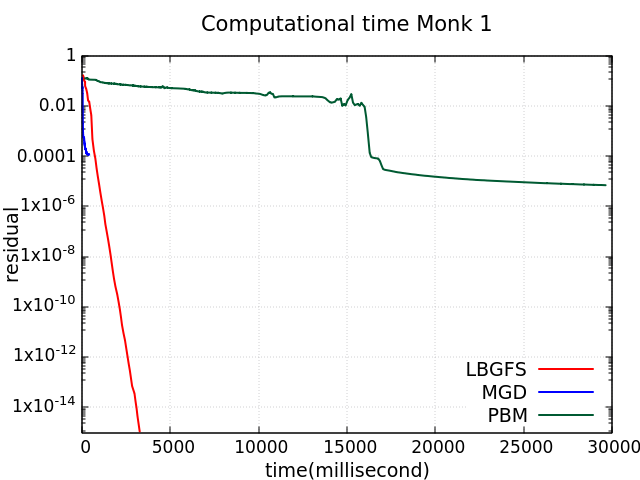
\includegraphics[width=\linewidth]{data/Comparison/Monk1/Monk1_CT_Comparison_log_standard.png}
		\subcaption{Standard}
	\end{minipage}%
	\begin{minipage}[t]{0.5\linewidth}
		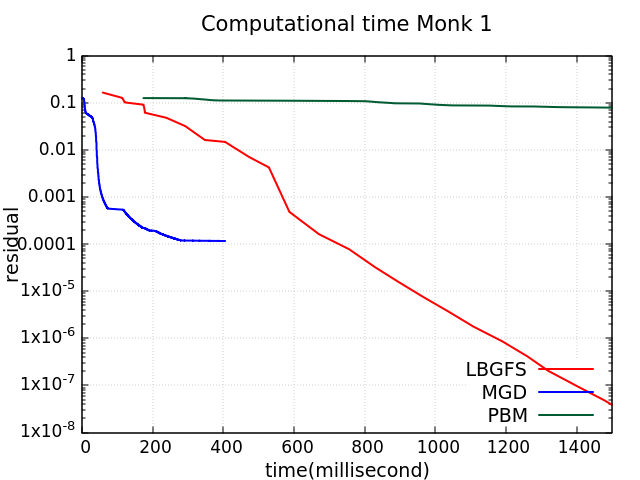
\includegraphics[width=\linewidth]{data/Comparison/Monk1/Monk1_CT_Comparison_log_zoom.png}
		\subcaption{Zoom}
	\end{minipage}
	\caption{Computational time comparison Monk 1 of configurations defined in table \ref{tab:nets_comp}}
	\label{CT-Monk1}
\end{figure}
\begin{figure}[H]
	\centering
	\begin{minipage}[t]{0.5\linewidth}
		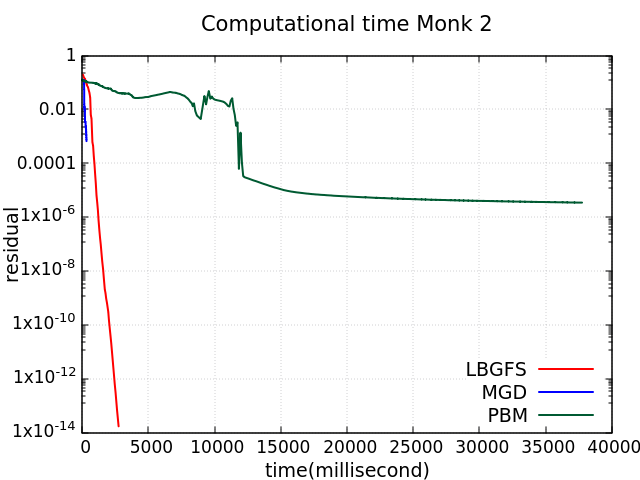
\includegraphics[width=\linewidth]{data/Comparison/Monk2/Monk2_CT_Comparison_log_standard.png}
		\subcaption{Standard}
	\end{minipage}%
	\begin{minipage}[t]{0.5\linewidth}
		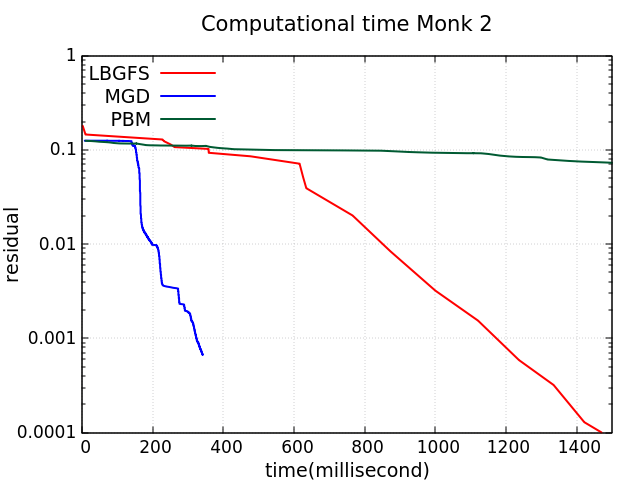
\includegraphics[width=\linewidth]{data/Comparison/Monk2/Monk2_CT_Comparison_log_zoom.png}
		\subcaption{Zoom}
	\end{minipage}
	\caption{Computational time comparison Monk 2 of configurations defined in table \ref{tab:nets_comp}}
	\label{CT-Monk2}
\end{figure}
\begin{figure}[H]
	\centering
	\begin{minipage}[t]{0.5\linewidth}
		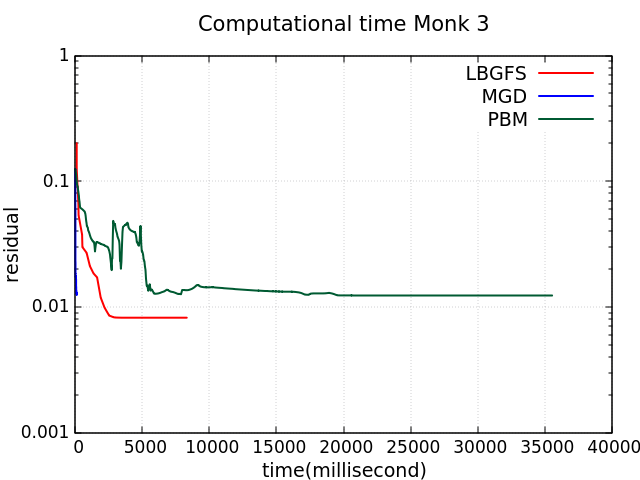
\includegraphics[width=\linewidth]{data/Comparison/Monk3/Monk3_CT_Comparison_log_standard.png}
		\subcaption{Standard}
	\end{minipage}%
	\begin{minipage}[t]{0.5\linewidth}
		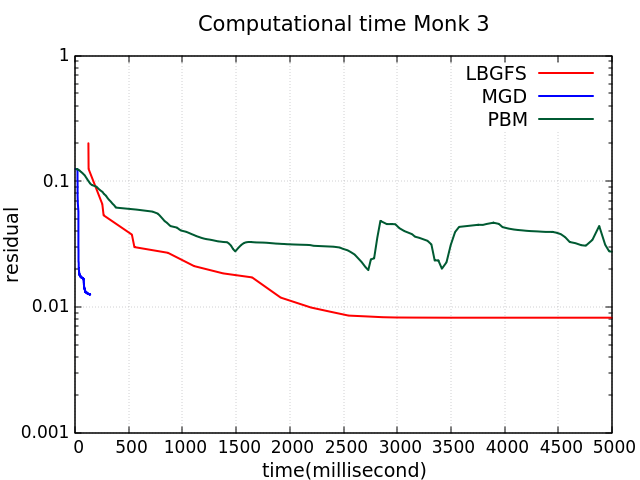
\includegraphics[width=\linewidth]{data/Comparison/Monk3/Monk3_CT_Comparison_log_zoom.png}
		\subcaption{Zoom}
	\end{minipage}
	\caption{Computational time comparison Monk 3 of configurations defined in table \ref{tab:nets_comp}}
	\label{CT-Monk3}
\end{figure}

\subsubsection{Gradient norm convergence speed}
\label{sec:gradient_norm_convergence_speed}
Here we can observe that the behaviour of the algorithms follows what we stated before in the theory about their convergence speed. We view from the plots that the norm of the gradient is not smooth in all the Monks dataset. In our opinion, this is due to the starting point of the training and the non-convexity of the objective function. We know from the theory that these methods tend to have some problems with the local minimum. Also, we can observe that at a certain point the norm tends to stabilize and converge to zero. Therefore, we can infer that in the neighbourhood of the last visited minima there are no other minimum better than itself and the search of the best minima can stop.
\begin{figure}[H]
	\centering
	\begin{minipage}[t]{0.5\linewidth}
		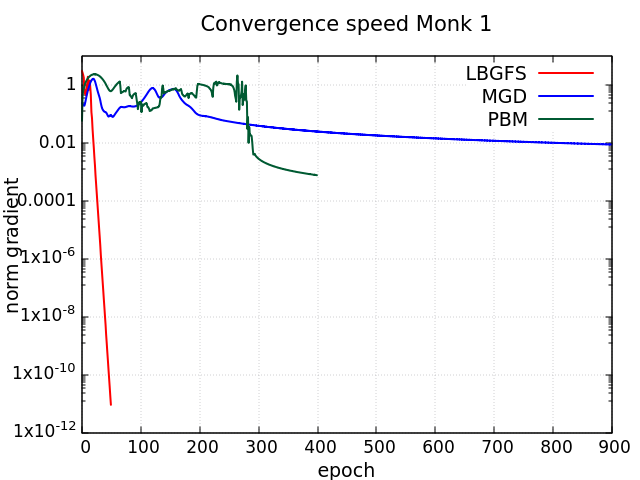
\includegraphics[width=\linewidth]{data/Comparison/Monk1/Monk1_CS_Comparison_log_standard.png}
		\subcaption{Standard}
	\end{minipage}%
	\begin{minipage}[t]{0.5\linewidth}
		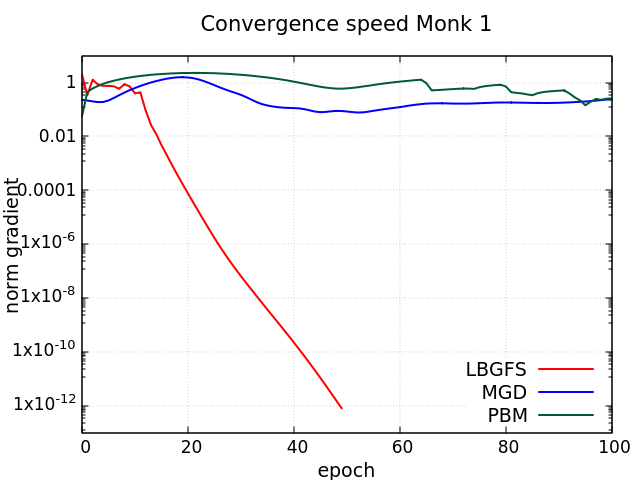
\includegraphics[width=\linewidth]{data/Comparison/Monk1/Monk1_CS_Comparison_log_zoom.png}
		\subcaption{Zoom}
	\end{minipage}
	\caption{Converge speed comparison Monk 1 of configurations defined in table \ref{tab:nets_comp}}
	\label{CS-Monk1}
\end{figure}
\begin{figure}[H]
	\centering
	\begin{minipage}[t]{0.5\linewidth}
		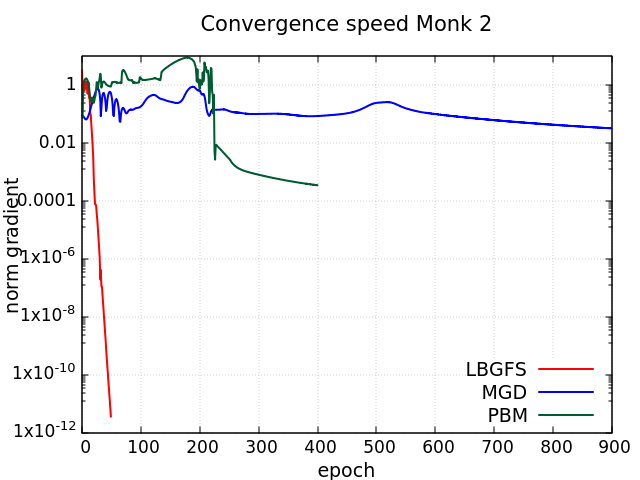
\includegraphics[width=\linewidth]{data/Comparison/Monk2/Monk2_CS_Comparison_log_standard.png}
		\subcaption{Standard}
	\end{minipage}%
	\begin{minipage}[t]{0.5\linewidth}
		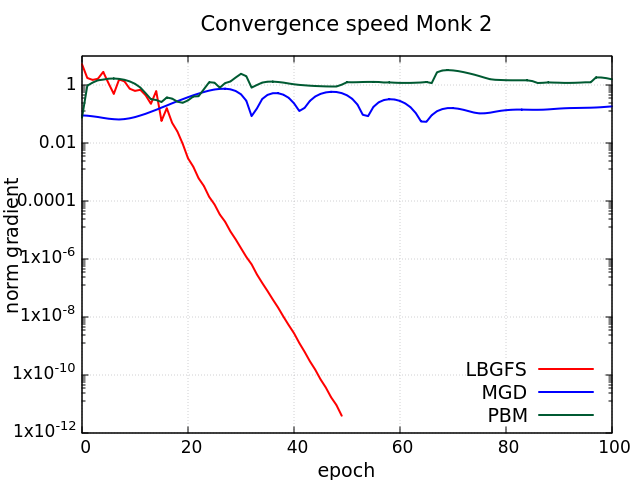
\includegraphics[width=\linewidth]{data/Comparison/Monk2/Monk2_CS_Comparison_log_zoom.png}
		\subcaption{Zoom}
	\end{minipage}
	 \caption{Converge speed comparison Monk 2 of configurations defined in table \ref{tab:nets_comp}}
	 \label{CS-Monk2}
\end{figure}
\begin{figure}[H]
	\centering
	\begin{minipage}[t]{0.5\linewidth}
		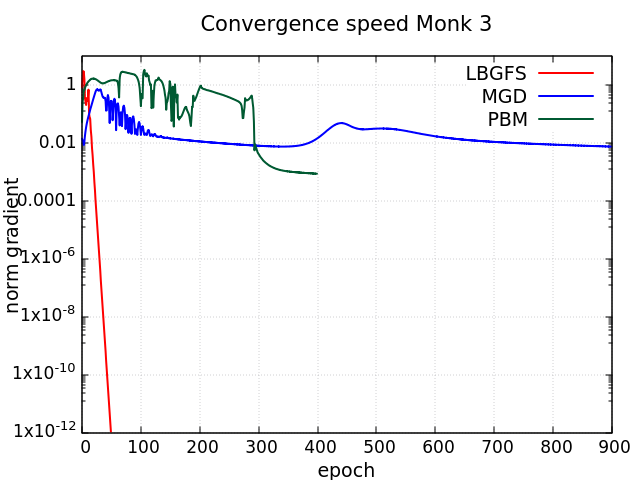
\includegraphics[width=\linewidth]{data/Comparison/Monk3/Monk3_CS_Comparison_log_standard.png}
		\subcaption{Standard}
	\end{minipage}%
	\begin{minipage}[t]{0.5\linewidth}
		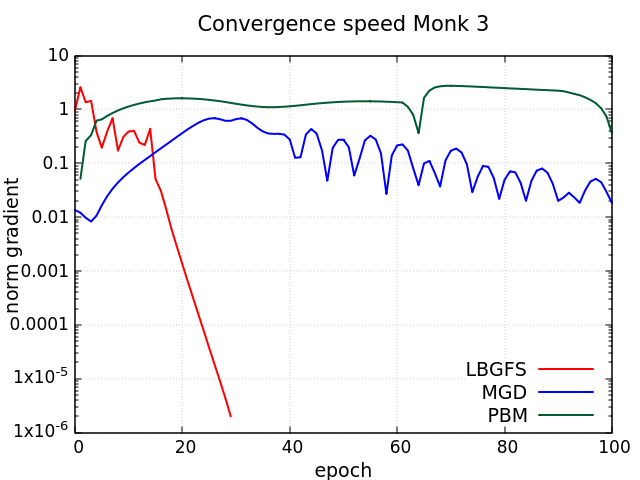
\includegraphics[width=\linewidth]{data/Comparison/Monk3/Monk3_CS_Comparison_log_zoom.png}
		\subcaption{Zoom}
	\end{minipage}
	\caption{Converge speed comparison Monk 3 of configurations defined in table \ref{tab:nets_comp}}
	\label{CS-onk3}
\end{figure}

\subsubsection{Residual error from $f^*$}
\label{sec:residual_error}
The residual value is obtained by the following formula: $ f(x_k) - f^*$ where  $f(x_{k})$ is the residual obtained at the iteration $k$ plus the  regularization term if it is used. The plots of the residual value obtained from the configurations in the table \ref{tab:nets_comp} are shown below. The residual curves obtained, also with an enlargement for each of them, are shown below.

\begin{figure}[H]
	\centering
	\begin{minipage}[t]{0.5\linewidth}
		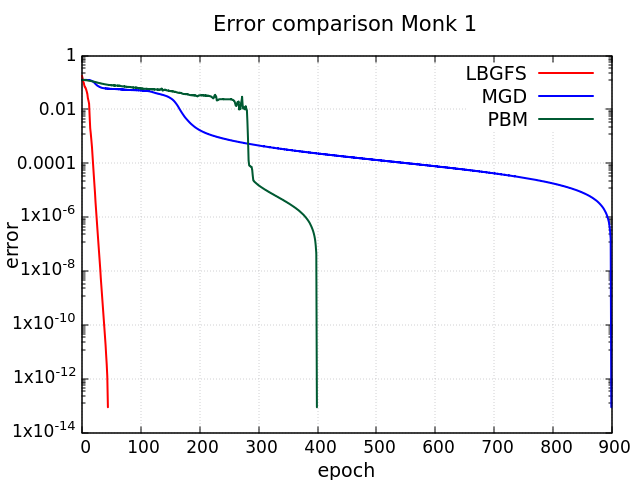
\includegraphics[width=\linewidth]{data/Comparison/Monk1/Monk1_R_Comparison_log_standard.png}
		\subcaption{Standard}
	\end{minipage}%
	\begin{minipage}[t]{0.5\linewidth}
		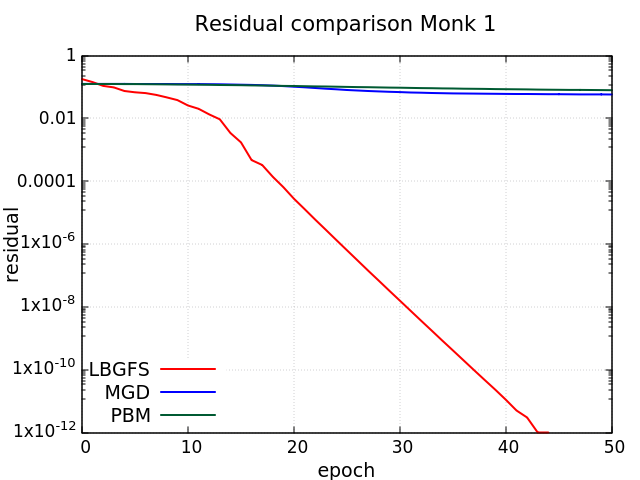
\includegraphics[width=\linewidth]{data/Comparison/Monk1/Monk1_R_Comparison_log_zoom.png}
		\subcaption{Zoom}
	\end{minipage}
	\caption{Residual comparison Monk 1 of configurations defined in table \ref{tab:nets_comp}}
	\label{R-Monk1}
\end{figure}
\begin{figure}[H]
	\centering
	\begin{minipage}[t]{0.5\linewidth}
		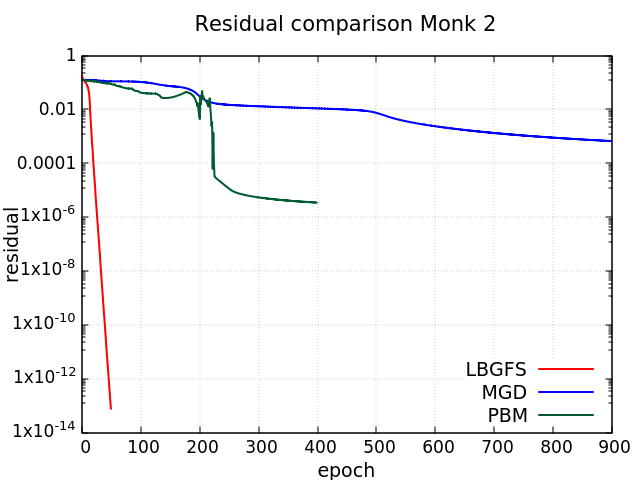
\includegraphics[width=\linewidth]{data/Comparison/Monk2/Monk2_R_Comparison_log_standard.png}
		\subcaption{Standard}
	\end{minipage}%
	\begin{minipage}[t]{0.5\linewidth}
		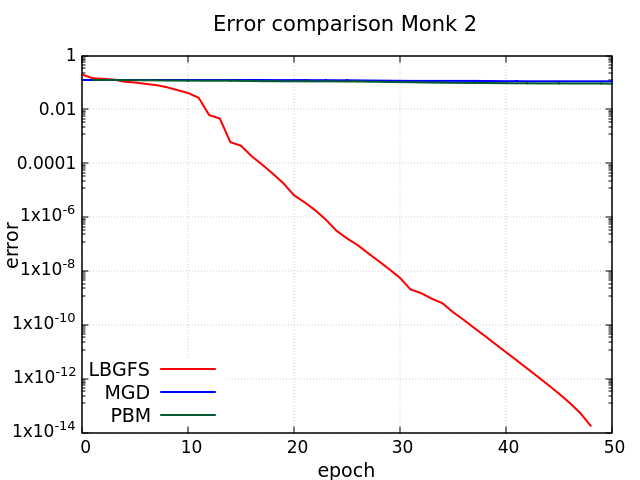
\includegraphics[width=\linewidth]{data/Comparison/Monk2/Monk2_R_Comparison_log_zoom.png}
		\subcaption{Zoom}
	\end{minipage}
	\caption{Residual comparison Monk 2 of configurations defined in table \ref{tab:nets_comp}}
	\label{R-Monk2}
\end{figure}
\begin{figure}[H]
	\centering
	\begin{minipage}[t]{0.5\linewidth}
		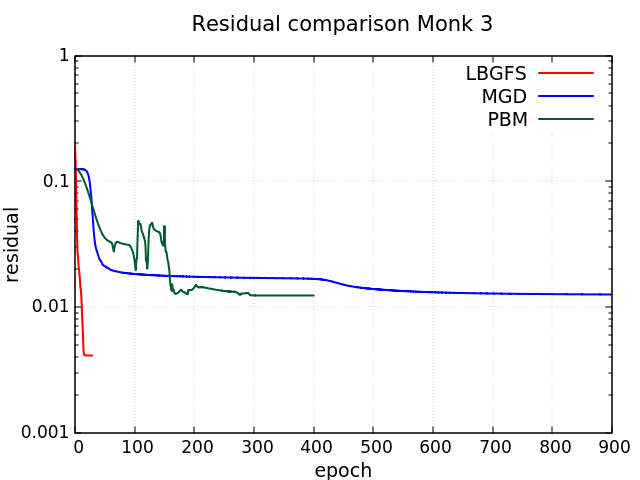
\includegraphics[width=\linewidth]{data/Comparison/Monk3/Monk3_R_Comparison_log_standard.png}
		\subcaption{Standard}
	\end{minipage}%
	\begin{minipage}[t]{0.5\linewidth}
		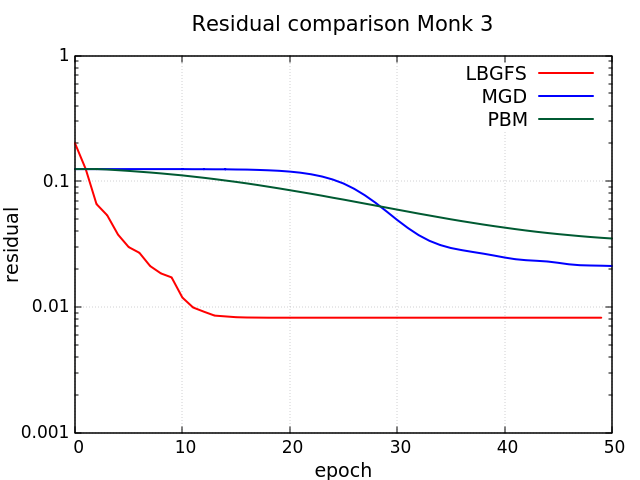
\includegraphics[width=\linewidth]{data/Comparison/Monk3/Monk3_R_Comparison_log_zoom.png}
		\subcaption{Zoom}
	\end{minipage}
	\caption{Residual comparison Monk 3 of configurations defined in table \ref{tab:nets_comp}}
	\label{R-Monk3}
\end{figure}